\begin{titlepage}

\centering

\begin{tikzpicture}

\node[opacity=0.3,inner sep=0pt,remember picture,overlay] at (4.5,-0.5){
\includegraphics[width= 0.8 \textwidth]{template/figures/jads_logo_grey.png}};

\node[inner sep=0pt] (logo) at (0,0)
    {
\includegraphics[width=.25\textwidth]{template/figures/jads_logo.png}};

\node[text width = 0.5\textwidth, right = of logo](title){\sffamily\huge\reporttitle};

\node[text width = 0.5\textwidth, yshift = 0.75cm, below = of title](subtitle){\sffamily\Large \reportsubtitle};

\gettikzxy{(subtitle.south)}{\sffamily\subtitlex}{\subtitley}
\gettikzxy{(title.north)}{\titlex}{\titley}
\draw[line width=1mm, Tue-red]($(logo.east)!0.5!(title.west)$) +(0,\subtitley) -- +(0,\titley);

\end{tikzpicture}
\vspace{3cm}

\sffamily\groupnumber

\vspace{1em}

{\sffamily\large
\begin{tabular}{ll}
\textbf{Full Name} & \textbf{Student ID}\\
\hline
\reportauthors
\end{tabular}
}

\vspace{1em}
\sffamily \grouptutor

\tikz[remember picture,overlay]\node[anchor=south,inner sep=0pt] at (current page.south) {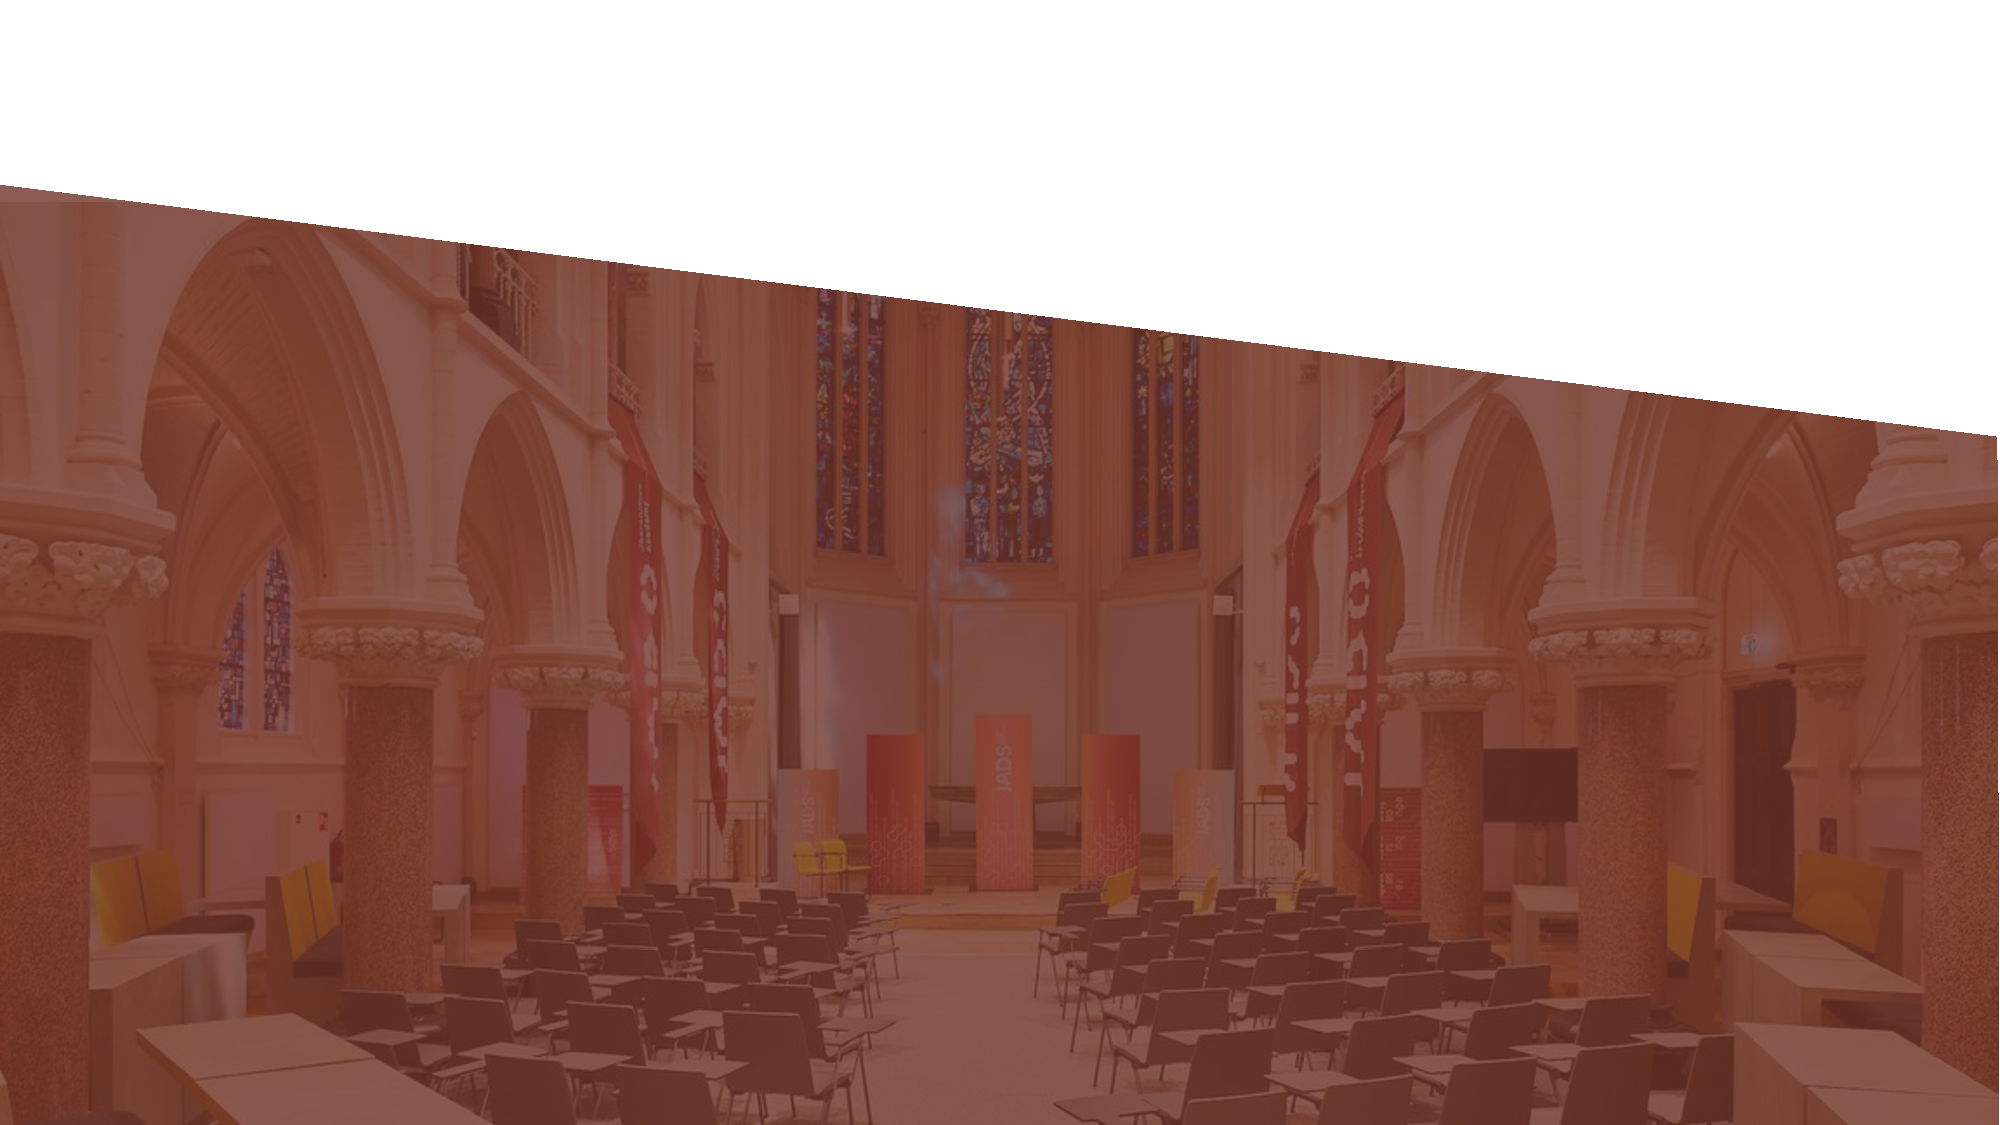
\includegraphics[width=\paperwidth]{template/figures/jads.pdf}};

\mbox{}
\vfill
\sffamily \Large \textcolor{white}{\placeanddate} \\

\end{titlepage}
\thispagestyle{empty}
